% Options for packages loaded elsewhere
\PassOptionsToPackage{unicode}{hyperref}
\PassOptionsToPackage{hyphens}{url}
%
\documentclass[
  ,man,floatsintext]{apa6}
\usepackage{amsmath,amssymb}
\usepackage{lmodern}
\usepackage{iftex}
\ifPDFTeX
  \usepackage[T1]{fontenc}
  \usepackage[utf8]{inputenc}
  \usepackage{textcomp} % provide euro and other symbols
\else % if luatex or xetex
  \usepackage{unicode-math}
  \defaultfontfeatures{Scale=MatchLowercase}
  \defaultfontfeatures[\rmfamily]{Ligatures=TeX,Scale=1}
\fi
% Use upquote if available, for straight quotes in verbatim environments
\IfFileExists{upquote.sty}{\usepackage{upquote}}{}
\IfFileExists{microtype.sty}{% use microtype if available
  \usepackage[]{microtype}
  \UseMicrotypeSet[protrusion]{basicmath} % disable protrusion for tt fonts
}{}
\makeatletter
\@ifundefined{KOMAClassName}{% if non-KOMA class
  \IfFileExists{parskip.sty}{%
    \usepackage{parskip}
  }{% else
    \setlength{\parindent}{0pt}
    \setlength{\parskip}{6pt plus 2pt minus 1pt}}
}{% if KOMA class
  \KOMAoptions{parskip=half}}
\makeatother
\usepackage{xcolor}
\usepackage{graphicx}
\makeatletter
\def\maxwidth{\ifdim\Gin@nat@width>\linewidth\linewidth\else\Gin@nat@width\fi}
\def\maxheight{\ifdim\Gin@nat@height>\textheight\textheight\else\Gin@nat@height\fi}
\makeatother
% Scale images if necessary, so that they will not overflow the page
% margins by default, and it is still possible to overwrite the defaults
% using explicit options in \includegraphics[width, height, ...]{}
\setkeys{Gin}{width=\maxwidth,height=\maxheight,keepaspectratio}
% Set default figure placement to htbp
\makeatletter
\def\fps@figure{htbp}
\makeatother
\setlength{\emergencystretch}{3em} % prevent overfull lines
\providecommand{\tightlist}{%
  \setlength{\itemsep}{0pt}\setlength{\parskip}{0pt}}
\setcounter{secnumdepth}{-\maxdimen} % remove section numbering
% Make \paragraph and \subparagraph free-standing
\ifx\paragraph\undefined\else
  \let\oldparagraph\paragraph
  \renewcommand{\paragraph}[1]{\oldparagraph{#1}\mbox{}}
\fi
\ifx\subparagraph\undefined\else
  \let\oldsubparagraph\subparagraph
  \renewcommand{\subparagraph}[1]{\oldsubparagraph{#1}\mbox{}}
\fi
\newlength{\cslhangindent}
\setlength{\cslhangindent}{1.5em}
\newlength{\csllabelwidth}
\setlength{\csllabelwidth}{3em}
\newlength{\cslentryspacingunit} % times entry-spacing
\setlength{\cslentryspacingunit}{\parskip}
\newenvironment{CSLReferences}[2] % #1 hanging-ident, #2 entry spacing
 {% don't indent paragraphs
  \setlength{\parindent}{0pt}
  % turn on hanging indent if param 1 is 1
  \ifodd #1
  \let\oldpar\par
  \def\par{\hangindent=\cslhangindent\oldpar}
  \fi
  % set entry spacing
  \setlength{\parskip}{#2\cslentryspacingunit}
 }%
 {}
\usepackage{calc}
\newcommand{\CSLBlock}[1]{#1\hfill\break}
\newcommand{\CSLLeftMargin}[1]{\parbox[t]{\csllabelwidth}{#1}}
\newcommand{\CSLRightInline}[1]{\parbox[t]{\linewidth - \csllabelwidth}{#1}\break}
\newcommand{\CSLIndent}[1]{\hspace{\cslhangindent}#1}
\ifLuaTeX
\usepackage[bidi=basic]{babel}
\else
\usepackage[bidi=default]{babel}
\fi
\babelprovide[main,import]{english}
% get rid of language-specific shorthands (see #6817):
\let\LanguageShortHands\languageshorthands
\def\languageshorthands#1{}
% Manuscript styling
\usepackage{upgreek}
\captionsetup{font=singlespacing,justification=justified}

% Table formatting
\usepackage{longtable}
\usepackage{lscape}
% \usepackage[counterclockwise]{rotating}   % Landscape page setup for large tables
\usepackage{multirow}		% Table styling
\usepackage{tabularx}		% Control Column width
\usepackage[flushleft]{threeparttable}	% Allows for three part tables with a specified notes section
\usepackage{threeparttablex}            % Lets threeparttable work with longtable

% Create new environments so endfloat can handle them
% \newenvironment{ltable}
%   {\begin{landscape}\centering\begin{threeparttable}}
%   {\end{threeparttable}\end{landscape}}
\newenvironment{lltable}{\begin{landscape}\centering\begin{ThreePartTable}}{\end{ThreePartTable}\end{landscape}}

% Enables adjusting longtable caption width to table width
% Solution found at http://golatex.de/longtable-mit-caption-so-breit-wie-die-tabelle-t15767.html
\makeatletter
\newcommand\LastLTentrywidth{1em}
\newlength\longtablewidth
\setlength{\longtablewidth}{1in}
\newcommand{\getlongtablewidth}{\begingroup \ifcsname LT@\roman{LT@tables}\endcsname \global\longtablewidth=0pt \renewcommand{\LT@entry}[2]{\global\advance\longtablewidth by ##2\relax\gdef\LastLTentrywidth{##2}}\@nameuse{LT@\roman{LT@tables}} \fi \endgroup}

% \setlength{\parindent}{0.5in}
% \setlength{\parskip}{0pt plus 0pt minus 0pt}

% Overwrite redefinition of paragraph and subparagraph by the default LaTeX template
% See https://github.com/crsh/papaja/issues/292
\makeatletter
\renewcommand{\paragraph}{\@startsection{paragraph}{4}{\parindent}%
  {0\baselineskip \@plus 0.2ex \@minus 0.2ex}%
  {-1em}%
  {\normalfont\normalsize\bfseries\itshape\typesectitle}}

\renewcommand{\subparagraph}[1]{\@startsection{subparagraph}{5}{1em}%
  {0\baselineskip \@plus 0.2ex \@minus 0.2ex}%
  {-\z@\relax}%
  {\normalfont\normalsize\itshape\hspace{\parindent}{#1}\textit{\addperi}}{\relax}}
\makeatother

\makeatletter
\usepackage{etoolbox}
\patchcmd{\maketitle}
  {\section{\normalfont\normalsize\abstractname}}
  {\section*{\normalfont\normalsize\abstractname}}
  {}{\typeout{Failed to patch abstract.}}
\patchcmd{\maketitle}
  {\section{\protect\normalfont{\@title}}}
  {\section*{\protect\normalfont{\@title}}}
  {}{\typeout{Failed to patch title.}}
\makeatother

\usepackage{xpatch}
\makeatletter
\xapptocmd\appendix
  {\xapptocmd\section
    {\addcontentsline{toc}{section}{\appendixname\ifoneappendix\else~\theappendix\fi\\: #1}}
    {}{\InnerPatchFailed}%
  }
{}{\PatchFailed}
\keywords{cognitive control, inhibition, antisaccade task, processing speed}
\usepackage{csquotes}
\usepackage{bm}
\usepackage{pcl}
\usepackage{amsmath}
\usepackage{setspace}
\ifLuaTeX
  \usepackage{selnolig}  % disable illegal ligatures
\fi
\IfFileExists{bookmark.sty}{\usepackage{bookmark}}{\usepackage{hyperref}}
\IfFileExists{xurl.sty}{\usepackage{xurl}}{} % add URL line breaks if available
\urlstyle{same} % disable monospaced font for URLs
\hypersetup{
  pdftitle={What Does the Antisaccade Task Measure?},
  pdfauthor={Jeffrey N. Rouder1, Adriana F. Chávez De la Peña1, Michael S. Pratte2, Virginia M. Richards1, Maggie C. Hernan3, Maeve M. Pascoe3, \& Anjali Thapar3},
  pdflang={en-EN},
  pdfkeywords={cognitive control, inhibition, antisaccade task, processing speed},
  hidelinks,
  pdfcreator={LaTeX via pandoc}}

\title{What Does the Antisaccade Task Measure?}
\author{Jeffrey N. Rouder\textsuperscript{1}, Adriana F. Chávez De la Peña\textsuperscript{1}, Michael S. Pratte\textsuperscript{2}, Virginia M. Richards\textsuperscript{1}, Maggie C. Hernan\textsuperscript{3}, Maeve M. Pascoe\textsuperscript{3}, \& Anjali Thapar\textsuperscript{3}}
\date{}


\shorttitle{Antisaccade Task}

\authornote{

Author Contributions: JNR conceived the project, programmed the experiment, and wrote the paper. AFCdlP performed the latent variable analysis in JAGS and edited the paper.MSP performed the complementary latent-variable analysis in lavaan and co-wrote the paper. VMR provided the adaptive staircase algorithms and analysis, and edited the paper. MCH and MMP collected the data. AT conceived the project, set up the experiments, organized the running of participants, and edited the paper. JNR was supported by NSF 2126976.

Open Science Practices: All code and data used in performing this research are publicly available at \url{https://github.com/PerceptionAndCognitionLab/inh-newtasks/blob/public/papers/as/v3/p.Rmd}. This Rmarkdown version provides the text; constructs figures, notes, and references; loads and cleans the data; and performs the analyses. The links therein refer to raw data, which are curated at github.com/amthapar/data-east/tree/main/antiSaccade/as12. Python code used to run the experiments is also available at this repository.

Correspondence concerning this article should be addressed to Jeffrey N. Rouder, Department of Cognitive Science, University of California, Irvine, CA, 92697. E-mail: \href{mailto:jrouder@uci.edu}{\nolinkurl{jrouder@uci.edu}}

}

\affiliation{\vspace{0.5cm}\textsuperscript{1} University of California, Irvine\\\textsuperscript{2} Mississippi State University\\\textsuperscript{3} Bryn Mawr College}

\abstract{%
One of the most popular and influential measures of cognitive control is the antisaccade task where participants identify briefly presented and subsequently masked targets at a peripheral location. Prior to mask presentation, there is a cue at an opposing location that must be inhibited. We assess the degree to which antisaccade accuracy reflects an inbhibition component independent of processing-speed by comparing performance to that in a prosaccade accuracy condition. Target durations in both tasks are adjusted with an adaptive 2-down/1-up staircase to produce constant accuracies. Individual target durations in the antisaccade condition are highly correlated to those in the prosaccade condition (\(r=.83\)). With a series of hierarchical models, we show there is but a single source of systemic variation across the conditions. We conclude that individual variation in inhibition in the antisaccade task is due to individual variation in processing speed.
}



\begin{document}
\maketitle

In psychology it is common to use the related concepts of \emph{cognitive control}, \emph{inhibition}, \emph{executive function}, and \emph{self regulation} to construct theories of attention, intelligence, working memory, development, aging, and psychopathology. The \emph{structure} of cognitive control, therefore, has been a central, cross-domain topic for over three decades. There have been a number of competing views of cognitive control. One popular position is that cognitive control is a common, domain-general, unified concept that is engaged in many tasks (Engle, Tuholski, Laughlin, \& Conway, 1999; Kane, Bleckley, Conway, \& Engle, 2001). Alternatives to this position come in two varieties. One is a finer subdivision of these general abilities including the proactive-vs-reactive dual-process model of Braver (2012), and the exceedingly popular three-factor model of Miyake et al. (2000). The other variety is that cognitive control does not exist in a general form; instead it is comprised of several, independent, domain-specific abilities (Rey-Mermet, Gade, \& Oberauer, 2018).

One main-line behavioral approach to exploring the structure of cognitive control is to apply latent variable models to individual performance scores. A brief summary is as follows: Individuals complete a battery of cognitive control exercises such as the Stroop task (Stroop, 1935), the flanker task (Eriksen \& Eriksen, 1974), the antisaccade task (Kane et al., 2001), the N-back memory task (Cohen et al., 1994), and the stop-signal task (Logan \& Cowan, 1984; Verbruggen et al., 2019). Then, the covariation across scores is decomposed into latent variables (Bollen, 1989; Skrondal \& Rabe-Hesketh, 2004). The relations among these latent variables purportedly reveal the underlying structure of cognitive control processes.

Results from latent-variable analyses have not been as conclusive or convincing as one might hope. The problem is that several of the experimental tasks which supposedly measure cognitive control do not correlate well with each other. For example, the correlation between flanker and Stroop effects in large studies is often near zero and never greater than .25 (Rouder, Haaf, \& Kumar, in preparation). It is difficult to determine whether these low correlations reflect a true lack of underlying correlation or attenuation from excessive measurement error (Hedge, Powell, \& Sumner, 2018; Rouder \& Haaf, 2019). Additionally, extant latent-variable analyses with cognitive-control tasks have been shown to be computationally unreliable (Karr et al., 2018).

Why are the correlations so low across scores? It is useful to partition cognitive control scores into those from \emph{tasks} and those from \emph{measures}. Tasks are true experiments where Donders' subtractive logic (Donders, 1868) is used to localize a process of interest. Two conditions are constructed where the only difference between them is that the process of interest loads more highly on to one than the other. The contrast of the conditions allows for a measure of the process free from nuisance factors. An example is the Stroop task where cognitive control is needed more for the incongruent than the congruent condition, and the subtraction provides a measure of cognitive control free from factors such as overall speed or motivation. Measures are instruments that do not have conditions nor use Donders' subtraction method. Cognitive-control measures include antisaccade accuracy, card-sorting performance and working-memory span. Performance typically reflects the composite of several skills and processes including but not limited to cognitive control.

The problem in measuring cognitive control has been with tasks. As several researchers have shown, the resulting difference scores are excessively variable even when there are 100s of trials per condition per participant (Draheim, Mashburn, Martin, \& Engle, 2019; Hedge et al., 2018; Rouder et al., in preparation). The statistical bright spot has been with measures. Because measures do not involve a subtraction, they tend to have higher reliability in typically-sized sample (Draheim et al., 2019). The problem with measures, however, is their interpretation. Whether measures index cognitive control is more-or-less asserted \emph{prima facie} without recourse to experimental-manipulation logic. Researcher who use measures rely on their correlations with other purportedly similar measures to bolster their interpretability. For example, the correlation between working-memory span and antisaccade accuracy is interpreted as coming from a shared factor of cognitive control (Unsworth, Robison, \& Miller, 2021).

A laudable goal is to find tasks or measures that have good statistical properties and clearly index cognitive control. Perhaps the best candidate comes from the antisaccade paradigm shown in Figure \ref{fig:trial} (Kane et al., 2001; Unsworth et al., 2021). Here, the cue precedes the target, and cues and targets are presented on opposite sides of fixation. There is an automatic orientation to the cue (Guitton, Buchtel, \& Douglas, 1985), and this orientation response must be successfully inhibited to process the target before it is masked. In the antisaccade task, cognitive control is manifest as the ability to inhibit prepotent automatic orienting responses, and the performance to the target, then, reflects the degree of control. In this indirect version, where stimulus information is available only briefly before masking, the accuracy to the target serves as a suitable measure of performance. Individual differences in target accuracy are known to have good reliability and correlate moderately well with working memory, problem-solving ability and other cognitive control measures (Chuderski \& Jastrzębski, 2018; Friedman \& Miyake, 2004; Unsworth et al., 2021).

We emphasize that the antisaccade paradigm is a measure rather than a task as there is often no manipulation or contrast. It is possible to construct a task with both antisaccade and prosaccade conditions. The prosaccade condition, where the cue and target are at the same location, serves as a baseline where cognitive control---the inhibition of the prepotent response to the cue---is counterproductive. Hence, we assume that when participants are aware that they are in a prosaccade condition, as they are in the following between-block design, they have no reason to inhibit the prepotent orienting response. Individual differences in prosaccade accuracy are expected of course, and these may reflect differences in the speed to shift gaze to the target location and the speed to process briefly-flashed stimuli, or, more generically, \emph{processing speed} (Salthouse, 1996). Antisaccade accuracy presumably indexes not only processing speed but the ability to inhibit the prepotent orienting response as well. The contrast between the prosaccade and antisaccade condition then may be used to isolate this control component much the same way that the contrast between incongruent and congruent conditions are used to isolate inhibition of prepotent responses in the Stroop tasks.

Researchers occasionally run prosaccade and antisaccade accuracy conditions in their experiments with the former serving as practice or filler. Importantly, contrasts are not constructed from the conditions (e.g., Kane et al., 2001; Unsworth et al., 2021). The exception is Rey-Mermet et al. (2018) who tuned stimulus target duration for each participant in their antisaccade task from an adaptive staircase in a preceding prosaccade task. This tuning serves as a control for individual differences in the ability to identify briefly flashed targets.

Constructing a contrast between prosaccade and antisaccade conditions is beset with the following practical problem: In our studies, there is often no single target duration that works well for both prosaccade and antisaccade conditions. If the target duration is tuned for moderate performance in the prosaccade condition, then performance may be near floor in the antisaccade condition, and, if the target duration is tuned for moderate performance in the antisaccade condition, then performance may be near ceiling for the prosaccade condition. To mitigate this problem, we used a simple adaptive staircase procedure to adjust the target duration for each individual separately in the prosaccade and antisaccade conditions. With the 2-down/1-up procedure (Levitt, 1971; Treutwein, 1995), we were able to ascertain a characteristic target duration that corresponded to 71\% accuracy for each individual in each condition. The duration in the prosaccade condition indexes a processing speed component without inhibition of the prepotent eye-movement response; the duration in the antisaccade condition indexes a combination of processing speed and inhibition of prepotent eye-movement responses; and, perhaps, the contrast may serve as a suitable measure of cognitive control.

The key prediction is about the correlation among the prosaccade and antisaccade condition. Of course we expect some correlation as both the prosaccade and antisaccade task tap many of the same processes including how well individuals can process quickly flashed targets with backwards masking. But we should not expect too high of a correlation if the antisaccade task taps inhibition and variation in this inhibition component accounts for individual differences. But what if the correlation is quite high? Then the antisaccade performance can be well predicted from the prosaccade performance. In this case, it is difficult to interpret antisaccade performance as localizing inhibition of a prepotent response. Instead the antisaccade measure should be thought of as tapping the same processes as the prosaccade condition.

In the following experiment we use a between-block design in which participants performed in the same condition for 50 trials before alternating to the other condition. The other design choice would have been a within-block design where conditions could switch from trial to trial. The between-design choice has the following advantages: (i) it limits the possibility of a carry-over effect of inhibition from antisaccade trials to prosaccade trials, (ii) it eliminates any task-switching costs, (iii) it takes shorter to run as task-indicating cues are not required, and (iv) the antisaccade condition is similar to antisaccade-accuracy measures used in cognitive-control batteries (cf., Unsworth, Schrock, \& Engle, 2004).

\hypertarget{method}{%
\section{Method}\label{method}}

\textbf{Subjects.} Twenty-six students from Bryn Mawr College participated in exchange for course credit or \$10. This sample was the largest one we could obtain before the semester ended. Although a sample size of 26 is not recommended for correlational studies in general, the resulting correlations are quite high and the subsequent analyses confirm that the sample size is sufficient in this case to localize latent correlations.

\textbf{Apparatus.} Participants were run individually on a PC running Windows. The experiment was controlled by a Python 3.6 program using Psychopy 3 libraries (Peirce et al., 2019). The display was an ordinary 19'' LCD running with a resolution of \(1440 \times 900\) pixels\(^2\) at a refresh rate of 75hz.

\textbf{Design.} The main dependent measure of interest is the stimulus duration obtained in an adaptive staircase procedure. The main independent variable is whether the cue is located around the target (prosaccade condition) or whether the cue is located 180\(^\circ\) from the target (antisaccade condition). This variable was manipulated within participant and was blocked so that the participant always knew whether the trial was in the prosaccade or antisaccade condition.

\textbf{Procedure.} Participants were flashed either X or M as a target on each trial, and they had to indicate whether this target was an M or an X by depressing the corresponding key on a computer keyboard. The structure of an antisaccade trial is shown in Figure \ref{fig:trial}. The target was placed at a certain angle relative to fixation, with all angles equally likely. In the antisaccade task, the cue consisted of two radial segments at an angle 180\(^\circ\) from the target (as shown). For the prosaccade trials (not shown), the cue was presented at the same angle as the target. In pilot work, we confirmed that cues were sufficiently separated from targets as to not cause any meta-contrast masking effects. Timing of the events are shown in Figure \ref{fig:trial} with the last blank lasting until response. After that, participants were provided feedback. They heard a pleasant 2-tone sequence for correct responses and a longer, lower tone for error responses.

Staircasing followed a 2-down/1-up procedure where the increments were single refreshes at 75hz (13.3 ms). Experimental blocks were comprised of 50 trials. The initial target duration in antisaccade blocks was 120ms (9 frames); that in prosaccade blocks was 66.7 ms (5 frames). The first two blocks were designed as practice blocks to familiarize the participant with the task. They consisted of only 10 trials and the target duration was started at 267 ms (20 frames). The first of these was a prosaccade block; the second was an antisaccade block. These 2 practice blocks were followed with the six experimental blocks of 50 trials each described above. The order of these 6 blocks followed an ABBAB design: some participants performed an antisaccade block; other performed a prosaccade block first.

\begin{figure}
\centering
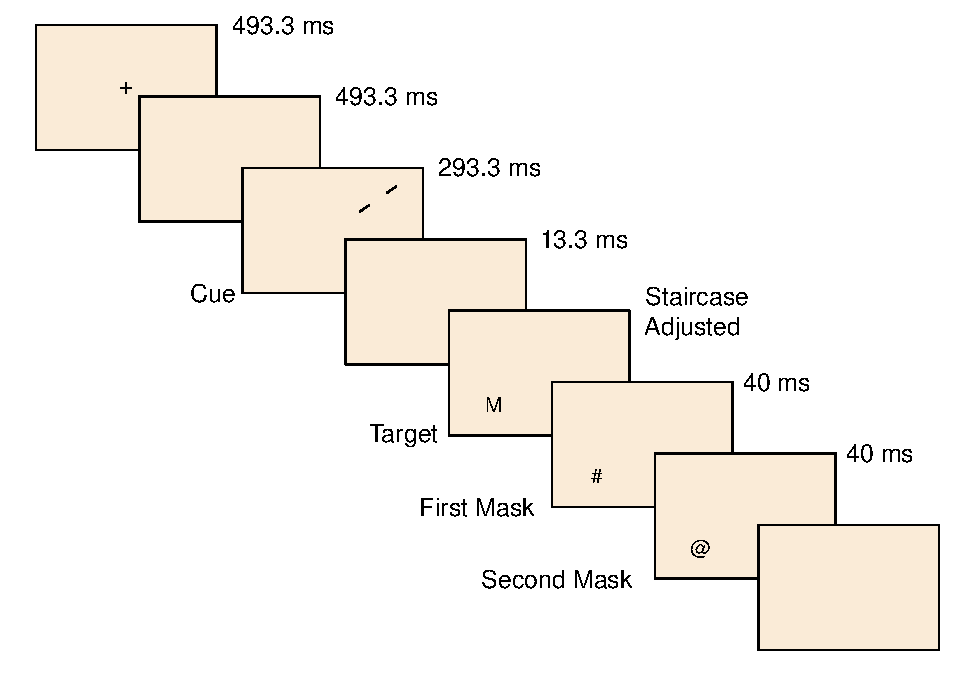
\includegraphics{p_files/figure-latex/trial-1.pdf}
\caption{\label{fig:trial}The structure and timing of an antisaccade trial. The cues were radial line segments at a certain angle relative to fixation. The targets were either X or M, and in the antisaccade trial, appeared opposite from the cue. The duration of the target was staircase adjusted, and the target was followed by a sequence of two masking displays. This sequence was highly effective and induced little response bias toward either target. Prosaccade trials were the same with the exception that the cue and target appeared at the same angle relative to fixation.}
\end{figure}

\hypertarget{results}{%
\section{Results}\label{results}}

\hypertarget{cleaning-steps}{%
\subsection{Cleaning Steps}\label{cleaning-steps}}

One participant was discarded because their staircases across all blocks increased without reaching any steady-state. This participant may have reversed the key mappings.

In the staircasing procedure, the goal is to describe the steady-state value after a transitory period from the initial value. There are a number of choices and we tried several options including discarding a fixed number of initial trials or discarding trials before a set number of reversals (Levitt, 1971). None of these choices had more than a marginal effect on the results. Herein, we discarded the first 15 trials of each 50-trial block and averaged the duration values on the remaining 35 trials to form a block score. Additionally, the first experimental block in each condition was discarded because learning effects were apparent for some participants. The results change only marginally if we include these two blocks.

\begin{figure}
\centering
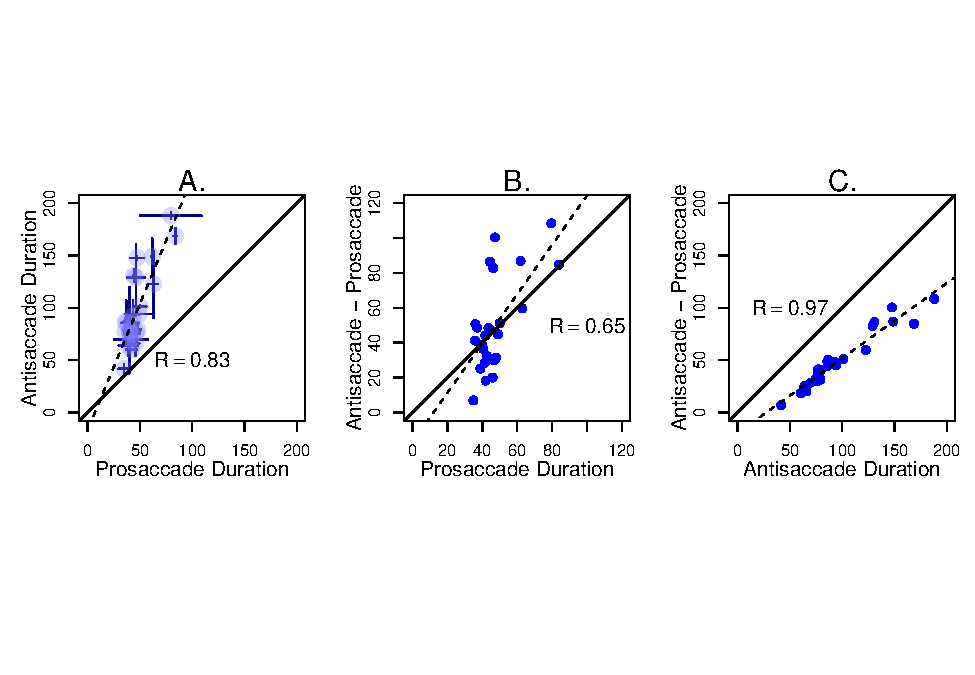
\includegraphics{p_files/figure-latex/scatter-1.pdf}
\caption{\label{fig:scatter}Relationship between prosaccade and antisaccade characteristic durations. A. Scatter of anti-sacade duration as a function of prosaccade duration. The high correlation is indicates that the antisaccade task is well predicted by the prosaccade task. Each point is comprised of two means, each across two blocks. The durations for the blocks are shown as segments. B. Scatter of the difference in durations across conditions as a function of prosaccade task duration. The positive correlation indicates that a cognitive-control component (defined as the contrast) is not independent from a processing-speed component. C. Scatter of the difference as a function of anti-saccade duration suggests that the tasks and the differences among them reflect a single factor.}
\end{figure}

\hypertarget{observed-relationships}{%
\subsection{Observed Relationships}\label{observed-relationships}}

Mean individual staircased durations for prosaccade and antisaccade tasks are shown as a scatter plot in Figure \ref{fig:scatter}A. Times for the antisaccade task were about twice as great as those for the prosaccade task reflecting the additional time needed to fixate the target's location when it was opposite the cue. There is a strong degree of correlation between the prosaccade and antisaccade task, \(r=0.83\) (95\% CI from 0.64 to 0.92).

The contrast between antisaccade and prosaccade durations provides a task-based localization of cognitive control. The relationship between this index and prosaccade performance is shown in Figure \ref{fig:scatter}B. There is a large degree of correlation here as well, \(r=0.65\). To the degree that this contrast localizes a cognitive-control process, it too is well predicted by processing speed in the prosaccade task. The remaining scatter plot, that between the contrast and the antisaccade duration performance is shown in Figure \ref{fig:scatter}C, and the exceedingly high correlation, \(r=0.97\), shows that the variability in the contrast reflects the variability in the antisaccade task more than variability in the prosaccade task.

\hypertarget{mixed-linear-models-to-assess-factor-structure-and-measurement-noise}{%
\subsection{Mixed Linear Models to Assess Factor Structure and Measurement Noise}\label{mixed-linear-models-to-assess-factor-structure-and-measurement-noise}}

The above correlation of .83 between prosaccade and antisaccade performance can be restated as follows: the prosaccade condition predicts about 70\% of the variance in the antisaccade condition. The critical question is about the remaining 30\%. On one hand, it could be the systematic variation across individuals in inhibition of prepotent eye-movement responses. If this possibility holds, then indeed the antisaccade accuracy task may be interpreted as reflecting individual differences in processing speed and cognitive control. On the other hand, however, the remaining 30\% of variation may be unaccounted measurement error. In this case, there is only one dimension or factor of systematic variation, and this dimension cannot be cognitive control as inhibition of the orienting cue is counterproductive in the prosaccade condition. In the current design, where each staircase in each condition is repeated within individuals, it is possible to assess whether this remaining 30\% is systematic variation with mixed linear models.

We construct a series of hierarchical models to account for measurement error and various systematic structures. The first model, \({\cal M}_1\), is an unstructured model to separate the two sources of variation. This first model is followed by two others with successive degrees of structure. The residual variabilities from the three models are compared much like one compares reduction in \(R^2\) from adding more covariates in linear models.

The unstructured model, \({\cal M}_1\) is:
\[ \begin{aligned}
{\cal M}_1:\quad & Y_{ijk} \sim \mbox{N}(\mu_{ij},\sigma_j^2)\\
&\mu_{ij} \sim \mbox{N}(\nu,\delta^2)
\end{aligned}
\]
\(Y_{ijk}\) is the staircased duration for the \(i\)th person in the \(j\)th condition (prosaccade/antisaccade) in the \(k\)th block. The latent variable \(\mu_{ij}\) is the ``true'' duration for the \(i\)th participant in the \(j\)th condition after measurement error, \(\sigma^2_j\) is accounted for. In the next stage, we treat \(\mu_{ij}\) as a random effect from a parent distribution, and this distribution has a mean \(\nu\) and variance \(\delta^2\). The key quantity here is \(\delta^2\)---it is the ``true'' variability across people and conditions after measurement error (\(\sigma^2\)) is accounted for. We expect \(\delta^2\) to be large in Model \({\cal M}_1\) as it accounts for variation across people and conditions. Indeed, under Model \({\cal M}_1\), \(\delta^2= 1094\)ms\(^2\), or, there is about 32.60 ms of deviations after modeling measurement error.\footnote{All models are implemented as a Bayesian model in JAGS (Denwood, 2016) using conventional hierarchical-modeling techniques (Rouder \& Province, 2019). We used weakly-informative priors that convey a minimum of information for this class of models (Haaf \& Rouder, 2017; Rouder \& Lu, 2005). For \({\cal M}_1\): \(\sigma^2\sim\) Inv-\(\chi^2\); \(\delta^2\sim\) Inv-\(\chi^2\); \(\nu\sim\mbox{Norm}(50,75^2)\), where the normal is parameterized in mean and variance. For \({\cal M}_2\): \(\sigma^2\sim\) Inv-\(\chi^2\); \(\delta^2\sim\) Inv-\(\chi^2\); \(\nu_j\sim\mbox{Norm}(50,75^2)\). For \({\cal M}_3\): \(\sigma^2\sim\) Inv-\(\chi^2\); \(\delta^2\sim\) Inv-\(\chi^2\); \(\nu_j\sim\mbox{Norm}(50,75^2)\); \(\lambda_j\sim\mbox{Norm}^+(30,50^2)\) where \(\mbox{Norm}^+\) is a normal truncated below at 0. MCMC chains were comprised of 20,000 iterations per model.}

To assess how much of this variance is accounted for by condition effects, we add condition effects to the model on \(\mu_{ij}\):
\[ \begin{aligned}
{\cal M}_2:\quad & Y_{ijk} \sim \mbox{N}(\mu_{ij},\sigma_j^2)\\
&\mu_{ij} \sim \mbox{N}(\nu_j,\delta^2)
\end{aligned}
\]
Here, the condition means \(\nu_1\) (prosaccade) and \(\nu_2\) (antisaccade) are allowed to vary resulting in a smaller residual variance. Under Model \({\cal M}_2\), \(\delta^2= 122.90\)ms\(^2\), which is much smaller than the original value under model \(\calM_1\) of 1,093.60. Dividing reveals that the condition effects in Model \({\cal M}_2\) accounts for about 88.80\% of the total variance in \(\mu_{ij}\). Indeed, there is a large difference in overall performance between the prosaccade and antisaccade conditions.

How much of this remaining variance may be accounted for by a one-factor structure? The one-factor model is:
\[ \begin{aligned}
{\cal M}_3:\quad & Y_{ijk} \sim \mbox{N}(\mu_{ij},\sigma_j^2)\\
&\mu_{ij} \sim \mbox{N}(\nu_j+\lambda_j\phi_i,\delta^2)\\
&\phi_i\sim\mbox{N}(0,1)
\end{aligned}
\]
In additional to condition means \(\nu_j\), there is a standardized characteristic duration for each person, \(\phi_i\), and condition loadings, \(\lambda_j\). To make the model identifiable, we restrict the loadings to be positive. This model is a hierarchical version of a standard one-factor model where cell means \(\mu_{ij}\) exhibit hierarchical shrinkage to the one-factor structure.

Under Model \({\cal M}_3\), \(\delta^2= 3.31\)ms\(^2\). Model \({\cal M}_3\) accounts for about 99.70\% of the unaccounted variance after modeling measurement error (that is, compared to Model \({\cal M}_1\)), and 97.31\% of the unaccounted variance after modeling measurement error and condition effects (that is, compared to Model \({\cal M}_2\)). Hence, there is not much residual variability to support a second factor.

\begin{figure}
\centering
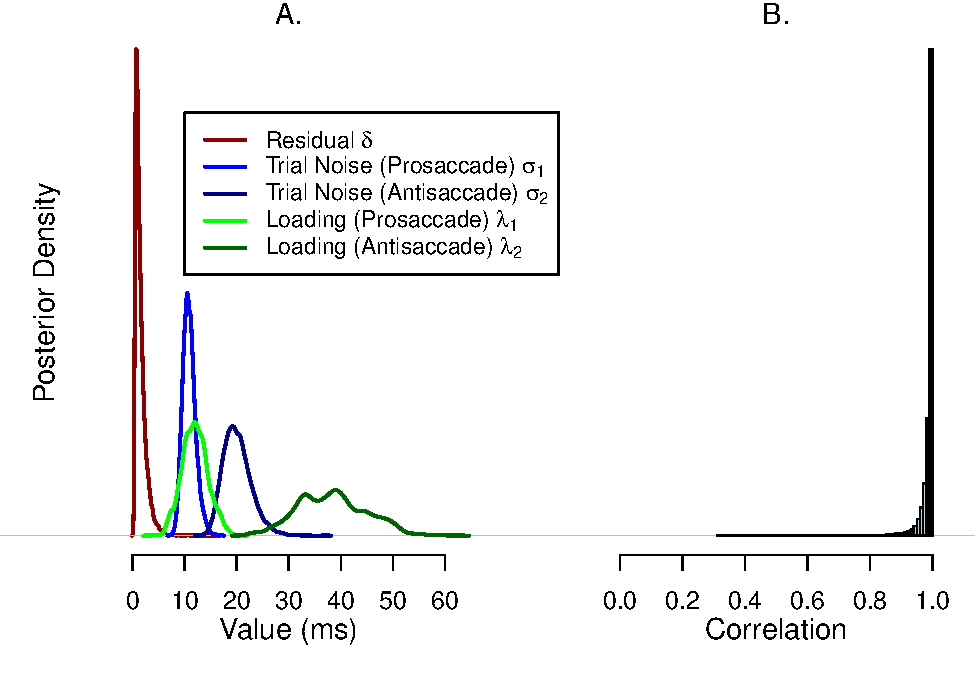
\includegraphics{p_files/figure-latex/mod3-1.pdf}
\caption{\label{fig:mod3}A. Posterior distribution of the standard deviation of the residual (red). For comparison, posteriors of measurement noise and task loadings are shown. B. Posterior of the latent correlation among prosaccade and antisaccade conditions.}
\end{figure}

A sense of the uncertainty in model parameters is shown in Figure \ref{fig:mod3}A. One critical parameter is the residual variance, \(\delta^2\), and plotted is the posterior of \(\delta\), the residual standard deviation, which, conveniently, is in units of milliseconds. Also plotted are standard deviations for trial noise (\(\sigma_1\) and \(\sigma_2\)) and task loadings (\(\lambda_1\) and \(\lambda_2\)), which are also in units of milliseconds. As can be seen, the posterior of the residual is well localized near zero and smaller than comparable parameters in the model. The posterior of the latent correlation between prosaccade and antisaccade performance is shown in Figure \ref{fig:mod3}B.\footnote{The latent correlation is the correlation of \(\mu_{ij}\) across conditions. It is expressed as a function of model parameters as \(\rho=\lambda_1\lambda_2/\sqrt{(\lambda_1^2+\delta^2)(\lambda_2^2+\delta^2)}\).} Once trial noise is accounted, the posterior mean of this correlation is 0.99 with 95\% credible interval from 0.92 to 1.00. Note that this latent correlation is far higher than the empirical correlation between conditions indicating that the previous value of .83 and the associated confidence intervals are somewhat attenuated by measurement noise (Spearman, 1904).

These model-based results show that almost all the systematic variance across individuals may be accounted for by a one-factor structure. As an additional check, we ran a confirmatory two-factor analysis with separate factors for the prosaccade and antisaccade conditions with durations from separate blocks entering into the analysis as separate manifest variables to enhance identifiability. The model converged well in Laavan (Rosseel, 2012), but resulted in a Heywood case (Rindskopf, 1984) where the resulting covariance matrix between the latent factors was not positive definite. The variances were too low for the degree of covariance indicating that the two latent factors were degenerate into a single latent factor. This Heywood case is not a technical issue but reflects deeper structure in the data. Consider the correlations among the blocks in the task. If there were two factors, we would expect a hypothetical pattern of correlations like that in Figure \ref{fig:heywood}A. Here, the two prosaccade blocks correlate well as they load onto one factor, and likewise for two antisaccade blocks as they load onto the other factor. The overall pattern is a familiar block diagonal pattern. The cross correlations across conditions reflect the correlations among the factors, but these can never be higher than the correlations within a condition. The observed correlations from the data are shown in Figure \ref{fig:heywood}B. Here the two prosaccade blocks correlate less well with each other (r=.4) than they do with each of the antisaccade blocks. This pattern cannot be accounted for with two separate factors for antisaccade and prosaccade blocks (Rindskopf, 1984). Conversely, the pattern is a signature of a single factor solution with a higher load in the antisaccade condition than in the prosaccade condition.

\begin{figure}
\centering
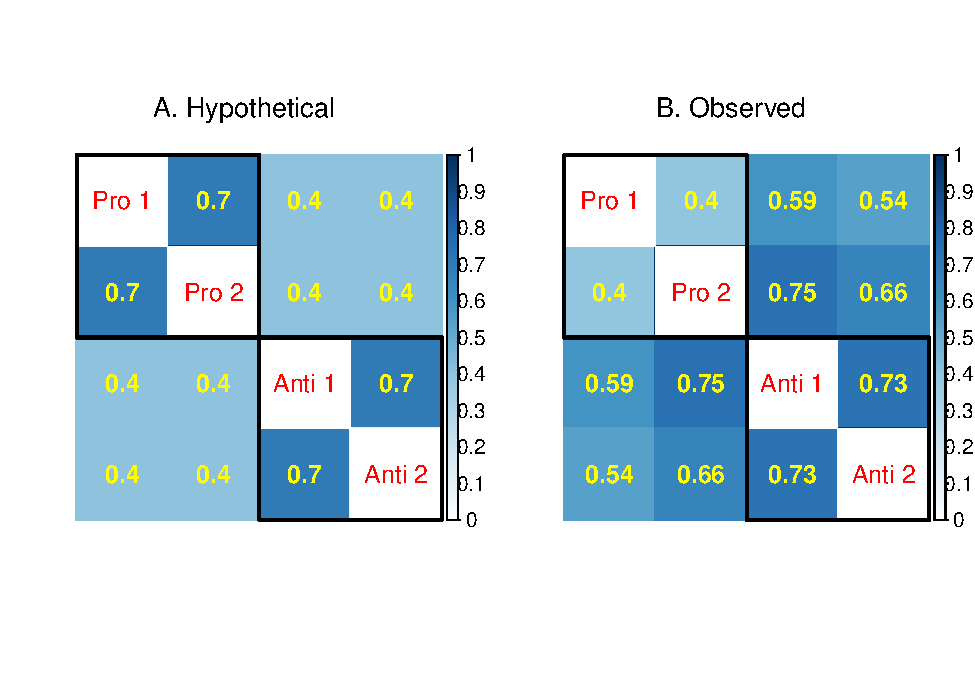
\includegraphics{p_files/figure-latex/heywood-1.pdf}
\caption{\label{fig:heywood}Correlation among the blocks. A. Hypothetical pattern from a two-factor setup shows a recognizable block-diagonal patter where the correlations across blocks from the same condition are higher than those from blocks across conditions. B. Correlations in the data do not have this block-diagonal pattern. The prosaccade blocks are less well correlated with each other than each is with the antisaccade blocks. This observed pattern is incompatible with a two-factor account.}
\end{figure}

These analyses converge on the same conclusion: individual differences in performance in the prosaccade and antisaccade conditions reflect variation on a single factor.

\hypertarget{conclusions}{%
\section{Conclusions}\label{conclusions}}

There are two critical results of the above study. First, not surprisingly, there was a large effect of condition. Thresholds were about twice as large in the antisaccade condition than the prosaccade condition indicating that the inhibition of prepotent response was time consuming. Second, even though there was a large effect, a single factor accounts for 97\% of the systematic individual variation across the conditions. Individual differences in the inhibition of the prepotent response reflect almost completely individual differences in processing speed.

How appealing is the concept of \emph{processing speed}? On one hand, processing speed has been an essential part of theories of intelligence and cognitive abilities (e.g., Carroll, 1993). Processing speed is often operationalized in the individual-differences literature as \emph{inspection time,} or the time needed to identify briefly-flashed and subsequently masked stimuli. And inspection time not only varies reliably across people, but correlates well with higher-order tasks such as working memory and intelligence tasks (Deary \& Stough, 1996; Jensen, 2006).

On the other hand, processing speed remains a vague concept. It is unclear how processing speed maps to theoretical concepts such as perception, representation, attention, or evidence accumulation. We highlight the recent work of Schubert, Hagemann, and Frischkorn (2017) as it addresses in part this gap. These researchers used the onset times of electrophysiological event-related components as proxies for various mental processes. The results were a positive manifold on individuals latent ERP components, that is, each individual had a characteristic latent processing time constant across the components. They concluded that this characteristic time likely reflects brain-wide differences in the efficiency of information transfer.

Processing speed, while characteristic of individual differences, is not the only factor that determines prosaccade and antisaccade performance. Some empirical manipulations have opposing effects on prosaccade and antisaccade performance. One example is the effect of the side of presentation in a monocular presentation (Kristjánsson, Vandenbroucke, \& Driver, 2004). Saccades are quicker to temporal-hemifield presentations than nasal-hemifield presentation in the prosaccade condition while quicker to nasal-hemifield presentations than temporal-hemifield presentation in the antisaccade condition. The result seemingly reflects an overall bias toward temporal hemifield movements. Another example comes from base-rate manipulations (Massen, 2004). Increasing the proportion of antisaccade trials in a mixed block both speeds eye-movement latencies for antisaccade trials and slows them for prosaccade trials. Hence, there are other processes in play, say faster eye movements to the periphery and sensitivity to expectations from base rates. Regardless, variation across individuals is highly correlated and concordant with a single factor indicating that variation in processing speed plays an outsized role.

In summary, our results show that researchers who study individual differences with antisaccade accuracy measures may have a difficult time with interpretation. The usual interpretation is that antisaccade indexes inhibition, perhaps independent of other factors. Yet, this task indexes a form of inhibition that is seemingly completely correlated with processing speed.

\newpage

\hypertarget{references}{%
\subsection*{References}\label{references}}
\addcontentsline{toc}{subsection}{References}

\hypertarget{refs}{}
\begin{CSLReferences}{1}{0}
\leavevmode\vadjust pre{\hypertarget{ref-Bollen.1989}{}}%
Bollen, K. A. (1989). \emph{Structural equations with latent variables}. {Wiley}.

\leavevmode\vadjust pre{\hypertarget{ref-Braver.2012}{}}%
Braver, T. S. (2012). The variable nature of cognitive control: A dual mechanisms framework. \emph{Trends in Cognitive Sciences}, \emph{16}(2), 106--113.

\leavevmode\vadjust pre{\hypertarget{ref-Carroll.1993}{}}%
Carroll, J. B. (1993). \emph{Human cognitive abilities: {A} survey of factor-analytic studies}. {Cambridge University Press}.

\leavevmode\vadjust pre{\hypertarget{ref-Chuderski.Jastrzebski.2018}{}}%
Chuderski, A., \& Jastrzębski, J. (2018). Much ado about aha!: {Insight} problem solving is strongly related to working memory capacity and reasoning ability. \emph{Journal of Experimental Psychology: General}, \emph{147}(2), 257--281. doi:\href{https://doi.org/10.1037/xge0000378}{10.1037/xge0000378}

\leavevmode\vadjust pre{\hypertarget{ref-Cohen.etal.1994}{}}%
Cohen, J. D., Forman, S. D., Braver, T. S., Casey, B. J., Servan-Schreiber, D., \& Noll, D. C. (1994). Activation of the prefrontal cortex in a nonspatial working memory task with functional {MRI}. \emph{Human Brain Mapping}, \emph{1}(4), 293--304. doi:\href{https://doi.org/10.1002/hbm.460010407}{10.1002/hbm.460010407}

\leavevmode\vadjust pre{\hypertarget{ref-Deary.Stough.1996}{}}%
Deary, I. J., \& Stough, C. (1996). Intelligence and inspection time: Achievements, prospects, and problems. \emph{American Psychologist}, \emph{51}(6), 599.

\leavevmode\vadjust pre{\hypertarget{ref-Denwood.2016}{}}%
Denwood, M. J. (2016). Runjags: {An R} package providing interface utilities, model templates, parallel computing methods and additional distributions for {MCMC} models in {JAGS}. \emph{Journal of Statistical Software}, \emph{71}, 1--25.

\leavevmode\vadjust pre{\hypertarget{ref-Donders.1868}{}}%
Donders, F. C. (1868). Die schnelligkeit psychischer processe: {Erster} artikel. \emph{Archiv Für Anatomie, Physiologie Und Wissenschaftliche Medicin}, 657--681.

\leavevmode\vadjust pre{\hypertarget{ref-Draheim.etal.2019}{}}%
Draheim, C., Mashburn, C. A., Martin, J. D., \& Engle, R. W. (2019). Reaction time in differential and developmental research: {A} review and commentary on the problems and alternatives. \emph{Psychological Bulletin}, \emph{145}(5), 508.

\leavevmode\vadjust pre{\hypertarget{ref-Engle.etal.1999}{}}%
Engle, R. W., Tuholski, S. W., Laughlin, J. E., \& Conway, A. R. A. (1999). Working {Memory}, {Short Term Memory}, and {General Fluid Intelligence}: {A} latent variable approach. \emph{Journal of Experimental Psychology: General}, \emph{128}, 309--331.

\leavevmode\vadjust pre{\hypertarget{ref-Eriksen.Eriksen.1974}{}}%
Eriksen, B. A., \& Eriksen, C. W. (1974). Effects of noise letters upon the identification of a target letter in a nonsearch task. \emph{Perception \& Psychophysics}, \emph{16}, 143--149.

\leavevmode\vadjust pre{\hypertarget{ref-Friedman.Miyake.2004}{}}%
Friedman, N. P., \& Miyake, A. (2004). The relations among inhibition and interference control functions: {A} latent-variable analysis. \emph{Journal of Experimental Psychology: General}, \emph{133}, 101--135.

\leavevmode\vadjust pre{\hypertarget{ref-Guitton.etal.1985}{}}%
Guitton, D., Buchtel, H. A., \& Douglas, R. M. (1985). Frontal lobe lesions in man cause difficulties in suppressing reflexive glances and in generating goal-directed saccades. \emph{Experimental Brain Research}, \emph{58}(3), 455--472.

\leavevmode\vadjust pre{\hypertarget{ref-Haaf.Rouder.2017}{}}%
Haaf, J. M., \& Rouder, J. N. (2017). Developing {Constraint} in {Bayesian Mixed Models}. \emph{Psychological Methods}, \emph{22}(4), 779--798.

\leavevmode\vadjust pre{\hypertarget{ref-Hedge.etal.2018}{}}%
Hedge, C., Powell, G., \& Sumner, P. (2018). The reliability paradox: {Why} robust cognitive tasks do not produce reliable individual differences. \emph{Behavioral Research Methods}.

\leavevmode\vadjust pre{\hypertarget{ref-Jensen.2006}{}}%
Jensen, A. R. (2006). \emph{Clocking the mind: {Mental} chronometry and individual differences}. {Elsevier}.

\leavevmode\vadjust pre{\hypertarget{ref-Kane.etal.2001}{}}%
Kane, M. J., Bleckley, M. K., Conway, A. R. A., \& Engle, R. W. (2001). A controlled-attention view of working-memory capacity. \emph{Journal of Experimental Psychology: General}, \emph{130}(2), 169--183. Retrieved from \url{http://search.ebscohost.com/login.aspx?direct=true\&db=psyh\&AN=2001-17501-002\&loginpage=Login.asp\&site=ehost-live\&scope=site}

\leavevmode\vadjust pre{\hypertarget{ref-Karr.etal.2018}{}}%
Karr, J. E., Areshenkoff, C. N., Rast, P., Hofer, S. M., Iverson, G. L., \& Garcia-Barrera, M. A. (2018). The unity and diversity of executive functions: {A} systematic review and re-analysis of latent variable studies. \emph{Psychological Bulletin}, \emph{144}(11), 1147.

\leavevmode\vadjust pre{\hypertarget{ref-Kristjansson.etal.2004}{}}%
Kristjánsson, Á., Vandenbroucke, M. W. G., \& Driver, J. (2004). When pros become cons for anti- versus prosaccades: Factors with opposite or common effects on different saccade types. \emph{Experimental Brain Research}, \emph{155}(2), 231--244. doi:\href{https://doi.org/10.1007/s00221-003-1717-9}{10.1007/s00221-003-1717-9}

\leavevmode\vadjust pre{\hypertarget{ref-Levitt.1971}{}}%
Levitt, H. (1971). Transformed {Up}‐{Down Methods} in {Psychoacoustics}. \emph{The Journal of the Acoustical Society of America}, \emph{49}, 467--477. doi:\href{https://doi.org/10.1121/1.1912375}{10.1121/1.1912375}

\leavevmode\vadjust pre{\hypertarget{ref-Logan.Cowan.1984}{}}%
Logan, G. D., \& Cowan, W. B. (1984). On the ability to inhibit thought and action: {A} theory of an act of control. \emph{Psychological Review}, \emph{91}(3), 295.

\leavevmode\vadjust pre{\hypertarget{ref-Massen.2004}{}}%
Massen, C. (2004). Parallel programming of exogenous and endogenous components in the antisaccade task. \emph{The Quarterly Journal of Experimental Psychology Section A}, \emph{57}(3), 475--498. doi:\href{https://doi.org/10.1080/02724980343000341}{10.1080/02724980343000341}

\leavevmode\vadjust pre{\hypertarget{ref-Miyake.etal.2000}{}}%
Miyake, A., Friedman, N. P., Emerson, M. J., Witzki, A. H., Howerter, A., \& Wager, T. D. (2000). The unity and diversity of executive functions and their contributions to complex {``frontal lobe''} tasks: {A} latent variable analysis. \emph{Cognitive Psychology}, \emph{41}(1), 49--100.

\leavevmode\vadjust pre{\hypertarget{ref-Peirce.etal.2019}{}}%
Peirce, J., Gray, J. R., Simpson, S., MacAskill, M., Höchenberger, R., Sogo, H., \ldots{} Lindeløv, J. K. (2019). {PsychoPy2}: {Experiments} in behavior made easy. \emph{Behavior Research Methods}, \emph{51}(1), 195--203. doi:\href{https://doi.org/10.3758/s13428-018-01193-y}{10.3758/s13428-018-01193-y}

\leavevmode\vadjust pre{\hypertarget{ref-Rey-Mermet.etal.2018}{}}%
Rey-Mermet, A., Gade, M., \& Oberauer, K. (2018). Should {We Stop Thinking About Inhibition}? {Searching} for {Individual} and {Age Differences} in {Inhibition Ability}. \emph{Journal of Experimental Psychology: Learning, Memory, and Cognition}. Retrieved from \url{http://dx.doi.org/10.1037/xlm0000450}

\leavevmode\vadjust pre{\hypertarget{ref-Rindskopf.1984}{}}%
Rindskopf, D. (1984). Structural equation models: {Empirical} identification, {Heywood} cases, and related problems. \emph{Sociological Methods \& Research}, \emph{13}(1), 109--119.

\leavevmode\vadjust pre{\hypertarget{ref-Rosseel.2012}{}}%
Rosseel, Y. (2012). Lavaan: {An R} package for structural equation modeling. \emph{Journal of Statistical Software}, \emph{48}, 1--36.

\leavevmode\vadjust pre{\hypertarget{ref-Rouder.Haaf.2019}{}}%
Rouder, J. N., \& Haaf, J. M. (2019). A psychometrics of individual differences in experimental tasks. \emph{Psychonomic Bulletin and Review}, \emph{26}(2), 452--467. Retrieved from \url{https://doi.org/10.3758/s13423-018-1558-y}

\leavevmode\vadjust pre{\hypertarget{ref-Rouder.etal.inpreparation}{}}%
Rouder, J. N., Haaf, J. M., \& Kumar, A. (in preparationin preparation). \emph{Why {Most Studies} of {Individual Differences With Cognitive Tasks Are Bound To Fail}}.

\leavevmode\vadjust pre{\hypertarget{ref-Rouder.Lu.2005}{}}%
Rouder, J. N., \& Lu, J. (2005). An {Introduction} to {Bayesian Hierarchical Models} with an {Application} in the {Theory} of {Signal Detection}. \emph{Psychonomic Bulletin and Review}, \emph{12}, 573--604.

\leavevmode\vadjust pre{\hypertarget{ref-Rouder.Province.2019}{}}%
Rouder, J. N., \& Province, J. M. (2019). Bayesian {Hierarchical Models} in {Psychological Science}: {A Tutorial}. \emph{New Methods in Cognitive Psychology}, 32--66.

\leavevmode\vadjust pre{\hypertarget{ref-Salthouse.1996}{}}%
Salthouse, T. A. (1996). The processing speed theory of adult age differences in cognition. \emph{Psychological Review}, \emph{103}, 403--428.

\leavevmode\vadjust pre{\hypertarget{ref-Schubert.etal.2017}{}}%
Schubert, A.-L., Hagemann, D., \& Frischkorn, G. T. (2017). Is general intelligence little more than the speed of higher-order processing? \emph{Journal of Experimental Psychology: General}, \emph{146}(10), 1498.

\leavevmode\vadjust pre{\hypertarget{ref-Skrondal.Rabe-Hesketh.2004}{}}%
Skrondal, A., \& Rabe-Hesketh, S. (2004). \emph{Generalized {Latent Variable Modeling}: Multilevel, longitudinal, and structural equation models}. {Boca Raton}: {CRC Press}.

\leavevmode\vadjust pre{\hypertarget{ref-Spearman.1904a}{}}%
Spearman, C. (1904). The {Proof} and {Measurement} of {Association} between {Two Things}. \emph{American Journal of Psychology}, \emph{15}, 72--101. Retrieved from \url{https://www.jstor.org/stable/pdf/1412159.pdf}

\leavevmode\vadjust pre{\hypertarget{ref-Stroop.1935}{}}%
Stroop, J. R. (1935). Studies of interference in serial verbal reactions. \emph{Journal of Experimental Psychology}, \emph{18}, 643--662.

\leavevmode\vadjust pre{\hypertarget{ref-Treutwein.1995}{}}%
Treutwein, B. (1995). Adaptive {Psychophysical Procedures}. \emph{Vision Research}, \emph{35}, 2503--2522.

\leavevmode\vadjust pre{\hypertarget{ref-Unsworth.etal.2021}{}}%
Unsworth, N., Robison, M. K., \& Miller, A. L. (2021). On the relation between working memory capacity and the antisaccade task. \emph{Journal of Experimental Psychology: Learning, Memory, and Cognition}.

\leavevmode\vadjust pre{\hypertarget{ref-Unsworth.etal.2004}{}}%
Unsworth, N., Schrock, J. C., \& Engle, R. W. (2004). Working {Memory Capacity} and the {Antisaccade Task}: {Individual Differences} in {Voluntary Saccade Control}. \emph{Journal of Experimental Psychology: Learning, Memory, and Cognition}, \emph{30}, 1302--1321.

\leavevmode\vadjust pre{\hypertarget{ref-Verbruggen.etal.2019}{}}%
Verbruggen, F., Aron, A. R., Band, G. P., Beste, C., Bissett, P. G., Brockett, A. T., \ldots{} Boehler, C. N. (2019). A consensus guide to capturing the ability to inhibit actions and impulsive behaviors in the stop-signal task. \emph{eLife}, \emph{8}, e46323. doi:\href{https://doi.org/10.7554/eLife.46323}{10.7554/eLife.46323}

\end{CSLReferences}


\end{document}
